%%%%%%%% ICML 2018 EXAMPLE LATEX SUBMISSION FILE %%%%%%%%%%%%%%%%%

\documentclass{article}

% Recommended, but optional, packages for figures and better typesetting:
\usepackage{microtype}
\usepackage{graphicx}
\usepackage{subfigure}
\usepackage{booktabs} % for professional tables

% hyperref makes hyperlinks in the resulting PDF.
% If your build breaks (sometimes temporarily if a hyperlink spans a page)
% please comment out the following usepackage line and replace
% \usepackage{icml2018} with \usepackage[nohyperref]{icml2018} above.
\usepackage{hyperref}

% Attempt to make hyperref and algorithmic work together better:
\newcommand{\theHalgorithm}{\arabic{algorithm}}

% Use the following line for the initial blind version submitted for review:
\usepackage{icml2018}

% If accepted, instead use the following line for the camera-ready submission:
%\usepackage[accepted]{icml2018}

% The \icmltitle you define below is probably too long as a header.
% Therefore, a short form for the running title is supplied here:
\icmltitlerunning{Submission and Formatting Instructions for ICML 2018}

\begin{document}

\twocolumn[
\icmltitle{Submission and Formatting Instructions for \\
           International Conference on Machine Learning (ICML 2018)}

% It is OKAY to include author information, even for blind
% submissions: the style file will automatically remove it for you
% unless you've provided the [accepted] option to the icml2018
% package.

% List of affiliations: The first argument should be a (short)
% identifier you will use later to specify author affiliations
% Academic affiliations should list Department, University, City, Region, Country
% Industry affiliations should list Company, City, Region, Country

% You can specify symbols, otherwise they are numbered in order.
% Ideally, you should not use this facility. Affiliations will be numbered
% in order of appearance and this is the preferred way.
\icmlsetsymbol{equal}{*}

\begin{icmlauthorlist}
\icmlauthor{Aeiau Zzzz}{equal,to}
\icmlauthor{Bauiu C.~Yyyy}{equal,to,goo}
\icmlauthor{Cieua Vvvvv}{goo}
\icmlauthor{Iaesut Saoeu}{ed}
\icmlauthor{Fiuea Rrrr}{to}
\icmlauthor{Tateu H.~Yasehe}{ed,to,goo}
\icmlauthor{Aaoeu Iasoh}{goo}
\icmlauthor{Buiui Eueu}{ed}
\icmlauthor{Aeuia Zzzz}{ed}
\icmlauthor{Bieea C.~Yyyy}{to,goo}
\icmlauthor{Teoau Xxxx}{ed}
\icmlauthor{Eee Pppp}{ed}
\end{icmlauthorlist}

\icmlaffiliation{to}{Department of Computation, University of Torontoland, Torontoland, Canada}
\icmlaffiliation{goo}{Googol ShallowMind, New London, Michigan, USA}
\icmlaffiliation{ed}{School of Computation, University of Edenborrow, Edenborrow, United Kingdom}

\icmlcorrespondingauthor{Cieua Vvvvv}{c.vvvvv@googol.com}
\icmlcorrespondingauthor{Eee Pppp}{ep@eden.co.uk}

% You may provide any keywords that you
% find helpful for describing your paper; these are used to populate
% the "keywords" metadata in the PDF but will not be shown in the document
\icmlkeywords{Machine Learning, ICML}

\vskip 0.3in
]

% this must go after the closing bracket ] following \twocolumn[ ...

% This command actually creates the footnote in the first column
% listing the affiliations and the copyright notice.
% The command takes one argument, which is text to display at the start of the footnote.
% The \icmlEqualContribution command is standard text for equal contribution.
% Remove it (just {}) if you do not need this facility.

%\printAffiliationsAndNotice{}  % leave blank if no need to mention equal contribution
\printAffiliationsAndNotice{\icmlEqualContribution} % otherwise use the standard text.

\begin{abstract}
This document provides a basic paper template and submission guidelines.
Abstracts must be a single paragraph, ideally between 4--6 sentences long.
Gross violations will trigger corrections at the camera-ready phase.
\end{abstract}

\section{Introduction}\label{sec:introduction}
\section{Background}\label{sec:background}
\section{Methods}\label{sec:methods}


\subsection{Solving the risk sensitive POMDP}
Marecki \cite{marecki} showed that RSPOMDPs can be solved for arbitrary utility functions using \keyword{reverse value iteration} in Belief Wealth Space.
For this the original state space must be augmented two times:

\begin{figure}[H]
\begin {center}
\begin {tikzpicture}[-latex ,auto ,node distance =3cm and 3cm ,on grid,
semithick , state/.style ={ circle ,fill=black!20, maximum width =2 cm}]
\node[state] (A) [align=center] {Observation\\Time\\Space};
\node[state] (B) [right of=A,align=center] {Belief\\Time\\Space};
\node[state] (C) [right of=B,align=center] {Belief\\Wealth\\Space};

\path (A) edge [line width=1mm, align=center] node[left] {} (B);
\path (B) edge [line width=1mm,align=center] node[below =0.25 cm] {} (C);
\end{tikzpicture}
\end{center}
\end{figure}

First augmentation is done by describing the probability of being in the good state with a function $\phi(b,o)$ ~\autoref{m:belief-update}:

\begin{align}
    b' = \phi(b,o) := ()
\end{align}

This augmentation transforms the POMDP into a MDP.
Second augmentation ...
\section{Results}\label{sec:results}
\subsection{Solving the risk sensitive POMDP}

\normalsize
Marecki \cite{marecki} showed that RSPOMDPs can be solved for arbitrary utility functions using \textbf{reverse value iteration} in Belief Wealth Space.
For this the original state space must be augmented two times:

\begin{figure}
\begin {center}
\begin {tikzpicture}[-latex ,auto ,node distance =4cm and 2cm ,on grid,
semithick , state/.style ={ circle ,fill=black!20, minimum width =3 cm}]
\node[state] (A) [align=center] {Observation\\Time\\Space};
\node[state] (B) [right of=A,align=center] {Belief\\Time\\Space};
\node[state] (C) [right of=B,align=center] {Belief\\Wealth\\Space};


\path (A) edge [line width=2mm, align=center] node[left] {} (B);
\path (B) edge [line width=2mm,align=center] node[below =0.25 cm] {} (C);
\end{tikzpicture}
\end{center}
\end{figure}

\hspace{2cm}

\subsection{Value functions in belief wealth space}


\normalsize

\begin{figure}
    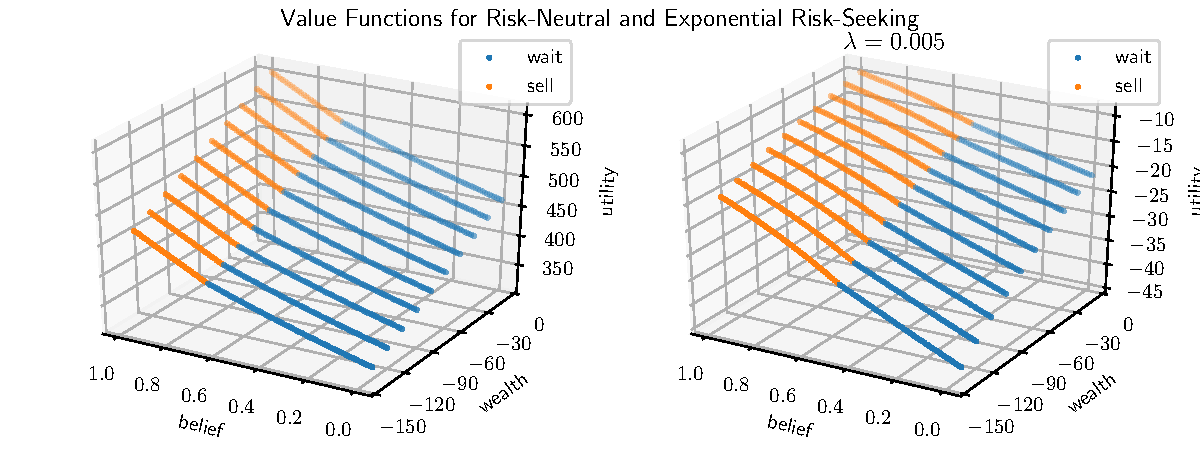
\includegraphics[width=0.98\linewidth]{img/exp_policy.pdf}\\
    \vspace{1cm}
    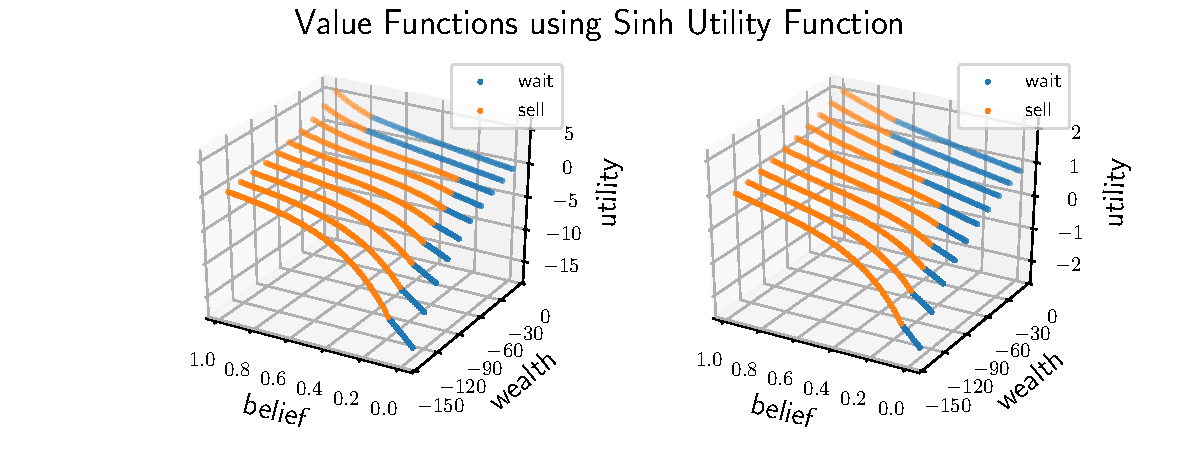
\includegraphics[width=0.98\linewidth]{img/sinh_policy.pdf}\\
    \vspace{1cm}
    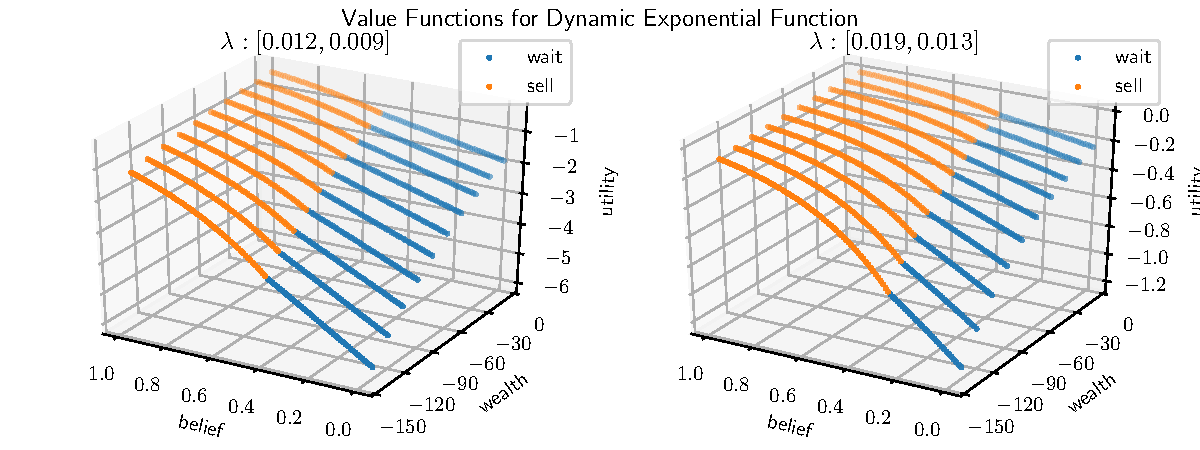
\includegraphics[width=0.98\linewidth]{img/dyn_policy.pdf}
    \caption{Value functions exhibiting different risk-behaviors; from top left: risk neutral agent (utility function is the identity function), risk-seeking agent with exponential utility function, two fixed time agents with different time thresholds, two agents with dynamic exponential utility function.}
\end{figure}

\subsection{From human behavior to utility functions}


\normalsize
\textbf{The original problem:}
\begin{itemize}
\item[①] Choose utility function with risk parameter.
\item[②] Perform value iteration.
\item[③] Derive policy.
\end{itemize}

\textbf{The inverse problem:}
\begin{itemize}
\item[①] Observe behavior.
\item[②] Estimate policy.
\item[③] Derive utility function and risk parameters.
\end{itemize}

The original problem is easy to solve, unfortunately for the inverse problem no solution is known. 

$\rightarrow$ Perform grid-search and choose optimal utility function.

\begin{figure}
    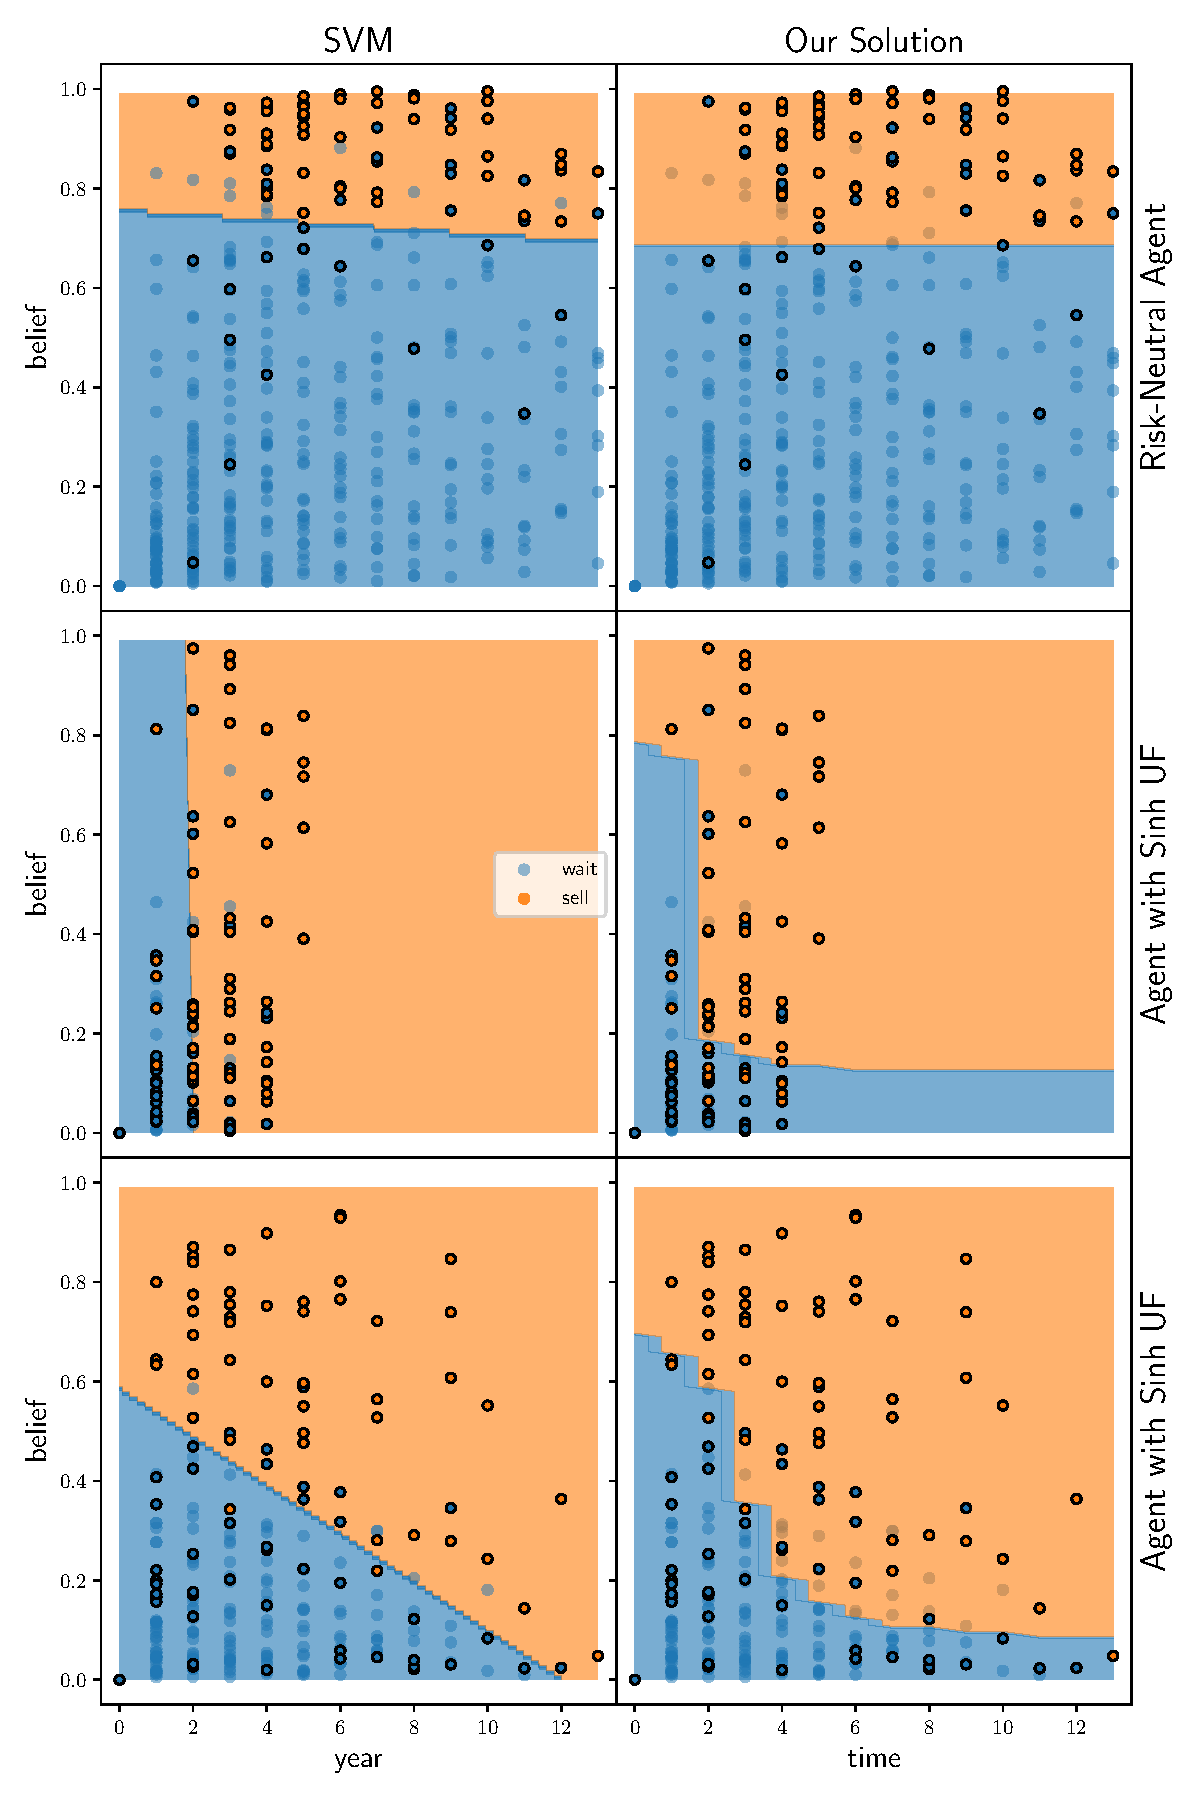
\includegraphics[width=0.8\linewidth]{img/fit}
    \caption{Examples from three human behaviors distinctly observed and replicated with RL agents. Behaviours by row: 1) Constant belief threshold, modelled by exponential utility, 2) Fixed time threshold, modelled by sinh utility, 3) Mixed strategy, modelled by dynamic exponential utility. Left column shows empirical optimal split of data using cross validation and linear kernel support vector machines, right column shows optimal policy found via gridsearch.}
    \label{fig:svm_vs_value}
\end{figure}

% TODO 6 boxes with only expensive expert and 3 behavior clusters.

\begin{figure}
% 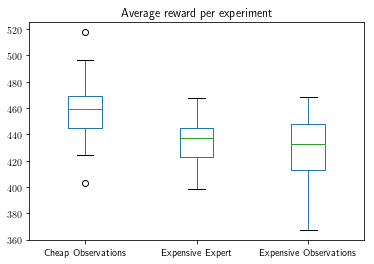
\includegraphics[width=0.4\linewidth]{img/avg_reward.png}
% 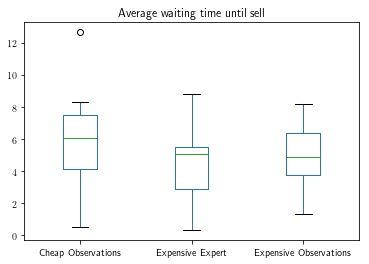
\includegraphics[width=0.4\linewidth]{img/avg_waiting.png}
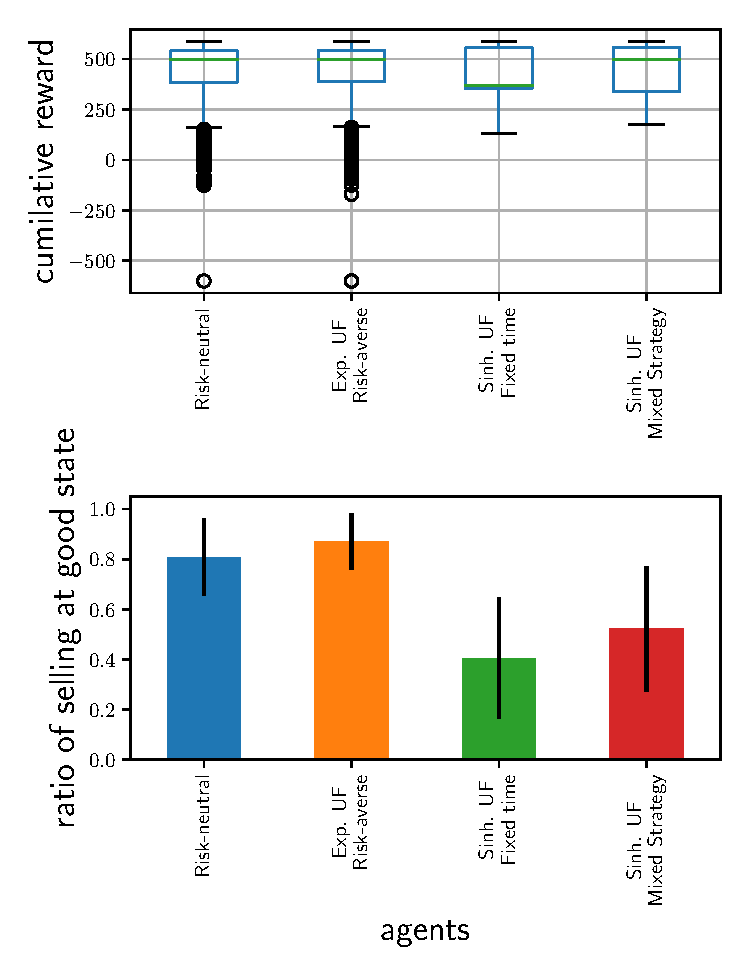
\includegraphics[width=0.8\linewidth]{img/performance.pdf}
\caption{Average reward and ratio of selling in the good state.}
\end{figure}


% Acknowledgements should only appear in the accepted version.
\section*{Acknowledgements}

\textbf{Do not} include acknowledgements in the initial version of
the paper submitted for blind review.

If a paper is accepted, the final camera-ready version can (and
probably should) include acknowledgements. In this case, please
place such acknowledgements in an unnumbered section at the
end of the paper. Typically, this will include thanks to reviewers
who gave useful comments, to colleagues who contributed to the ideas,
and to funding agencies and corporate sponsors that provided financial
support.


% In the unusual situation where you want a paper to appear in the
% references without citing it in the main text, use \nocite
\nocite{langley00}

\bibliography{example_paper}
\bibliographystyle{icml2018}


%%%%%%%%%%%%%%%%%%%%%%%%%%%%%%%%%%%%%%%%%%%%%%%%%%%%%%%%%%%%%%%%%%%%%%%%%%%%%%%
%%%%%%%%%%%%%%%%%%%%%%%%%%%%%%%%%%%%%%%%%%%%%%%%%%%%%%%%%%%%%%%%%%%%%%%%%%%%%%%
% DELETE THIS PART. DO NOT PLACE CONTENT AFTER THE REFERENCES!
%%%%%%%%%%%%%%%%%%%%%%%%%%%%%%%%%%%%%%%%%%%%%%%%%%%%%%%%%%%%%%%%%%%%%%%%%%%%%%%
%%%%%%%%%%%%%%%%%%%%%%%%%%%%%%%%%%%%%%%%%%%%%%%%%%%%%%%%%%%%%%%%%%%%%%%%%%%%%%%
\appendix
\section{Do \emph{not} have an appendix here}

\textbf{\emph{Do not put content after the references.}}
%
Put anything that you might normally include after the references in a separate
supplementary file.

We recommend that you build supplementary material in a separate document.
If you must create one PDF and cut it up, please be careful to use a tool that
doesn't alter the margins, and that doesn't aggressively rewrite the PDF file.
pdftk usually works fine. 

\textbf{Please do not use Apple's preview to cut off supplementary material.} In
previous years it has altered margins, and created headaches at the camera-ready
stage. 
%%%%%%%%%%%%%%%%%%%%%%%%%%%%%%%%%%%%%%%%%%%%%%%%%%%%%%%%%%%%%%%%%%%%%%%%%%%%%%%
%%%%%%%%%%%%%%%%%%%%%%%%%%%%%%%%%%%%%%%%%%%%%%%%%%%%%%%%%%%%%%%%%%%%%%%%%%%%%%%


\end{document}


% This document was modified from the file originally made available by
% Pat Langley and Andrea Danyluk for ICML-2K. This version was created
% by Iain Murray in 2018. It was modified from a version from Dan Roy in
% 2017, which was based on a version from Lise Getoor and Tobias
% Scheffer, which was slightly modified from the 2010 version by
% Thorsten Joachims & Johannes Fuernkranz, slightly modified from the
% 2009 version by Kiri Wagstaff and Sam Roweis's 2008 version, which is
% slightly modified from Prasad Tadepalli's 2007 version which is a
% lightly changed version of the previous year's version by Andrew
% Moore, which was in turn edited from those of Kristian Kersting and
% Codrina Lauth. Alex Smola contributed to the algorithmic style files.
